\chapter{Introduction}
\label{ch:introduction}
Conventional energy resources such as fossil fuels and nuclear energy are not only limited but also pose adverse effects on the environment. Therefore, we are striving to find a cheap and renewable source of energy. Wind energy is such source of energy, getting more popular and more affordable. Novel wind turbine designs such as the \indexAcron{Vertical-Axis Wind Turbine}{VAWT} are now a promising research field that can satisfy this growing demand.

	\begin{figure}[!b]
        \centering
        \begin{subfigure}[b]{0.25\textwidth}
                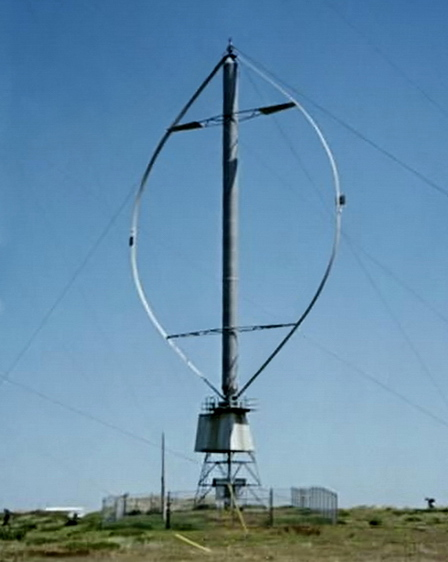
\includegraphics[height=0.2\textheight]{figures/introduction/Darrieus-windmill.jpg}
                \caption{VAWT: Darrieus wind turbine\cite{darrieusWindmill}}
                \label{fig:Darrieus-windmill}
        \end{subfigure}%
        \qquad \qquad%add desired spacing between images, e. g. ~, \quad, \qquad etc.
          %(or a blank line to force the subfigure onto a new line)
        \begin{subfigure}[b]{0.25\textwidth}
                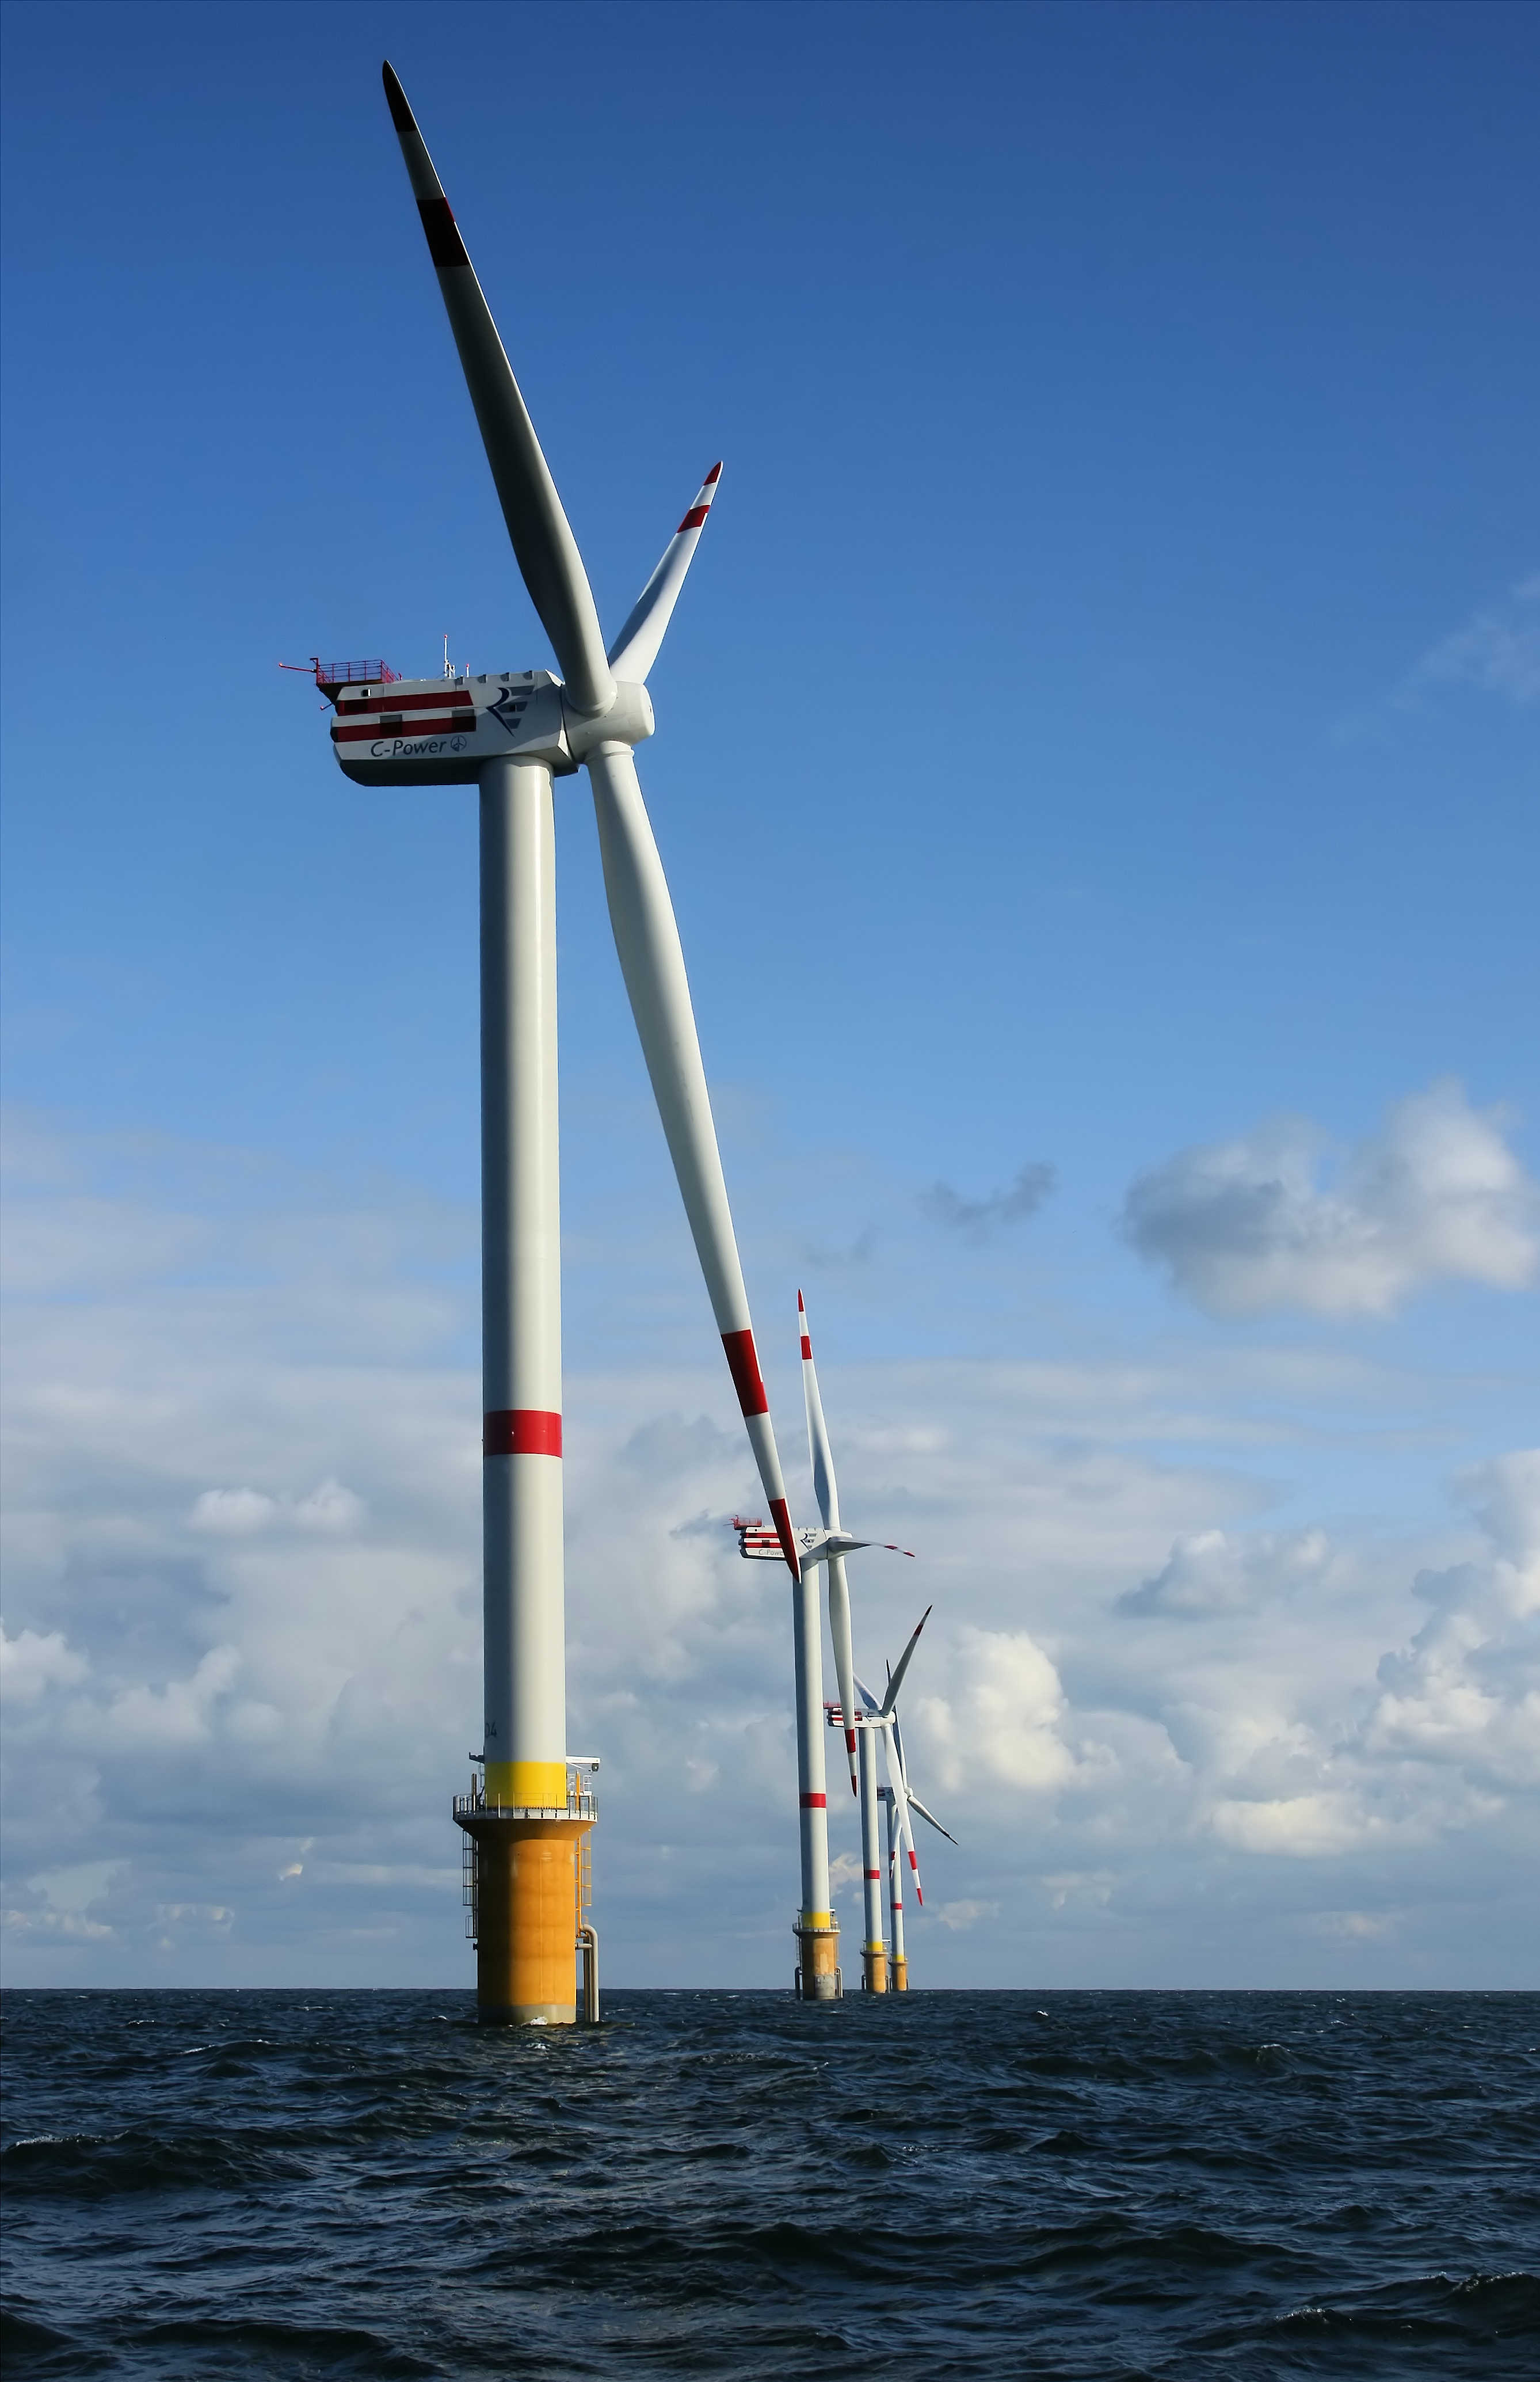
\includegraphics[height=0.2\textheight]{figures/introduction/HAWT_compressed.jpg}
                \caption{HAWT: Offshore wind turbine \cite{HAWTWindmill}}
                \label{fig:HAWT}
        \end{subfigure}
        \caption{VAWT vs. HAWT}
        \label{fig:VAWTvsHAWT}
	\end{figure}

VAWTs are unlike the normal wind turbines, which are mounted on a mast away from the ground and generate energy by spinning perpendicular to the ground, figure \ref{fig:VAWTvsHAWT}, whereas the \indexAcron{Horizontal-Axis Wind Turbine}{HAWT}, spins parallel to the ground with its hub located at the ground, figure \ref{fig:HAWT}. The VAWT has it's generator located at the ground, allowing it to be easily accessible and maintained. However, the main advantage is the early wake dissipation of VAWTs. Near-wake experiments of Ferreira (2009) \cite{SimaoFerreira2009}, and simulations of Vermeer (2003) \cite{Vermeer2003a} have shown that the fluid past the turbine is more turbulent. Due to this higher turbulence, the flow is able to recover much earlier than convectional wind turbines. This allows the turbines to be placed much closer, potentially outputting more power per ground. Furthermore, VAWTs operate independently of the flow direction, and can operate at low wind speeds (i.e. at low tip-speed ratios).

However, there are some limitations that we must take into account. As the blades pass through their own wake, complex wake-body interactions take place, figure \ref{fig:3DunsteadyPanelVAWT}. These have adverse effects on the blade structure, making it more susceptible to fatigue. As the blade is constantly pitching, flow behaviors such as dynamic stall and constant vortex shedding take place (Ferreira \cite{SimaoFerreira2008a}). These complex fluid behaviors makes it hard to predict the performance of a VAWTs and this is one of the reasons why VAWTs are not widely used. 

	\begin{figure}[!t]
		\centering
		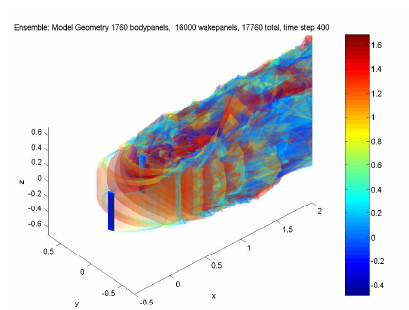
\includegraphics[width=0.6\linewidth]{figures/introduction/3DunsteadyPanelVAWT.png}
		\caption{3-D Unsteady Panel simulation of a Straight-bladed VAWT showing the strength of the shed vorticity. The VAWT blades interact with their own wake increasing the complexity of the wake geometry, source: Dixon et. al \cite{Dixon2008}.}
		\label{fig:3DunsteadyPanelVAWT}
	\end{figure}

In addition, a VAWT operates at a large Reynolds, number making accurate numerical methods computationally very expensive. So we see that we require a numerical method that can not only reproduce accurate results, but is also efficient at modeling the flow around the turbine.

\section{Motivation and Goal}
The goal of this research is to develop an efficient, reliable and accurate numerical method for modeling the flow around a \indexAcron{Two Dimensional}{2D} VAWT, enabling to compute the correct performance characteristics. The two approaches of investigating the flow around a turbine are by either using a numerical method to model the flow, or by performing an experimental test, for example in a wind tunnel.

To understand the unsteady aerodynamic behavior, \indexAcron{Particle Image Velocimetry}{PIV} has been a useful tool to visualize the flow around the turbine. PIV was used by Ferreira et al. (2007) \cite{Ferreira2007a}, showing that it is possible to measure the flow characteristics around the blade. The downside to experimental investigation is that it is very expensive to investigate all types of airfoil geometries, blade geometries and VAWT configurations. However, investigating this is vital in understanding the performance characteristics of VAWT. Furthermore, it is difficult to perform experiments on arrays of wind turbines in a wind tunnel.

Numerical methods are therefore a popular alternative as the cost of simulation is becoming progressively smaller, and the accuracy of the models is increasing day by day. \indexAcron{Actuator Disk}{AD} and \indexAcron{Blade Element Momentum}{BEM} models are the simplest models, built upon satisfying the momentum balance of the turbine with the fluid. The advantage is that they are very fast, however they lack the accuracy that is obtained by experimental simulation. Flow phenomena such as dynamic stall and flow separation cannot be modeled by these methods, and therefore we must rely on more powerful tools.

	\begin{figure}[!t]
		\centering
		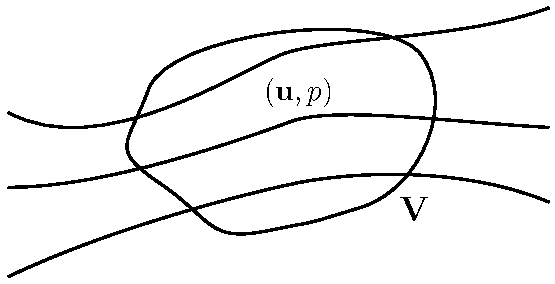
\includegraphics[width=0.6\linewidth]{figures/introduction/eulerianRF.pdf}
		\caption{Eulerian formulation of the fluid. We observe a given volume $\mathbf{V}$ and evaluate the change in properties of the fluid, velocity $\mathbf{u}$ and pressure $p$ at time passes.}
		\label{fig:eulerianRF}
	\end{figure}

To ensure more accuracy, one has to solve the Navier-Stokes equation of the flow around the turbine without large simplifications. \indexAcron{Computional Fluid Dynamics}{CFD} methods discretize the fluid into smaller cells (or volumes) and solve the Navier-Stokes equations. This type of formulation is known as an Eulerian formulation as we are evaluating the change in flow property in a given cell/volume, figure \ref{fig:eulerianRF}. In order to fully resolve the flow around the turbine, we would need a fine mesh near the blade where we have small scale vorticies. However, far from the body, where these vorticies dissipated into low frequency vortical structures, we can have lower mesh resolution. This means that at various regions of the flow, we require mesh resolutions of various magnitudes. This becomes a problem when we have moving boundaries as the mesh has to be adapted depending on the location of the body.

An alternative method is to use a Lagrangian formulation of the Navier-Stokes equations, known as vortex methods. These methods employ vorticity transport equations which makes them ideal for describing the evolution of the wake vorticity. Furthermore, they do not require cells/volumes to describe the domain. In addition, they use simulation acceleration methods such as \indexAcron{Fast Multipole Method}{FMM} and parallel computation in \indexAcron{Graphical Processing Units}{GPU} making them orders of magnitude faster than the typical CFD methods. However, vortex method cannot inherently take into account the solid body. They require additional methods that can describe the effect of the body in the fluid and the vorticity generated from the body.

	\begin{figure}[!t]
		\centering
		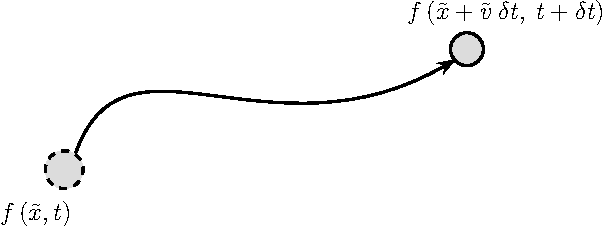
\includegraphics[width=0.6\linewidth]{figures/introduction/lagrangianRF2-crop.pdf}
		\caption{Lagrangian formulation of the fluid. We track the path of the individual fluid elements as time passes.}
		\label{fig:lagrangianRF}
	\end{figure}

We see that Eulerian method is accurate when describing the blade-wake interaction but not efficient when describing multi-scale domains. The Lagrangian method is very efficient in evolving the vorticity of the fluid. Due to auto-adaptive nature of the Lagrangian method, it is an ideal choice when describing the multi-scale flow characteristics. However, it is not efficient in resolving the near-body region, where the vorticity is generated. Therefore, in order to use the advantages of both methods, we have decided to use a domain-decomposition method, referred to as \indexAcron{Hybrid Eulerian-Lagrangian Vortex Particle Method}{HELVPM}. 

For the HELVPM, the Eulerian grid method will be used at the near-walls, and the Lagrangian vortex method will be used in the wake region. With the proper coupling of these methods, we can ensure that this numerical method can capture not only the near-wake phenomena such as vortex shedding, dynamic stall, and the wake-body interaction, but also the large-scale flow structures such as the evolution of the VAWT wake.

\section{Research Aim and Plan}

We have formulated a research that can help us accomplish our goal. The research questions that are derived from the goal of the project is as follows:

\paragraph*{Research Questions:}
	\begin{itemize}
	\item \textit{Is it possible to develop an efficient and accurate numerical method by an
	hybrid approach, with the vortex particle method solving the wake, and the Navier-Stokes grid solver solving the near-body region?}
	
	\item \textit{Will it be able to predict similar performance characteristics and flow phenomena as observed from the experiments?}
	
	\item \textit{Will it be capable of simulating the blade-wake interaction and the dynamic stall?}
	
	\item \textit{Where are the errors and what are their sources?}
	\end{itemize}
%\textit{Is it possible to develop an efficient and accurate numerical method by an
%hybrid approach; where the vortex particle method is used in the wake, and the Navier-Stokes grid solver is
%used at the near-body region? Will it be able to simulate real life performance characteristics of a Vertical-Axis Wind Turbine? Will it be able to predict similar performance characteristics and flow phenomena as observed from the wind tunnel experimental setup? Will it be capable of simulating the blade-wake interaction
%and the dynamic stall? Where are the errors and what are their sources?}

In order to answer the research questions, the goal of the project is to develop an efficient and accurate numerical method that is not only capable of capturing the small scale flow phenomena such as the dynamic stall and the vortex shedding, but is also efficient at modeling the evolution of the wake. Once the model has been developed, we will verify the approach and validate it against cases obtained from literature.

\paragraph*{Research aim and plan:}
\textit{
	\begin{itemize}
	\item Develop the hybrid method for capturing small-scale phenomena and large scale phenomena.
	\item Verify the efficiency, reliability, and the accuracy of the model.
	\item Verify and validate the model with test cases from literature.
	\end{itemize}
}
The innovativeness of this project is that such hybrid modeling has not been yet applied for the wind energy problem case. Through the parallelization of the vortex particle method in a GPU and employing solver acceleration techniques such as the FMM, this simulation could give an edge in the understanding the flow behavior of a VAWT.

\section{Verification and Validation Test Cases}
\label{sec:vavtc}
In order to assess the accuracy of this hybrid formulation, the following test cases have been used:

	\begin{description}
	\item[Lamb-Oseen vortex] \cite{Lamb1993} \cite{Tryggeson2007} \hfill\\
	Lamb-Oseen vortex test case is an analytical solution derived from the NS equation, and is a test case for unbounded flow (without any wall). This is the first model that will be used to validate the Lagrangian method and Eulerian method separately. As it describes an unbounded flow, we do not need to concern with the vorticity generation problem. This helps us focus on just the evolution of the vorticity field.
	\item[Clercx-Bruneau dipole] \cite{Clercx2006a}\hfill\\
	The Clercx-Bruneau dipole test case is the simple case of a colliding dipole with a wall. This test case will be used to verify and validate the coupling of the Eulerian and the Lagrangian method in the presence of a solid wall. This test case focuses on the interaction of vorticity with the wall making it ideal to verify and validate the proper generation of vorticity and its transfer to the Lagrangian subdomain.
	\item[Impulsively started cylinder] \cite{Koumoutsakos1995a} \cite{Chang1991} \cite{Braza1986} \cite{Lecointe1984}\hfill\\
	The impulsively started cylinder test case is used to analyze the forces acting on the cylinder. This test case is used to verify and validate the lift and drag evolution of the cylinder exposed to free-stream flow.
	\item[Elliptic Airfoil] \cite{Nair1997a}\hfill\\
	The elliptic airfoil test case focuses on the flow separation past a lifting body. The elliptic airfoil is pitched at high angle of attack and the flow past the airfoil is comparatively unsteady and undergoes phenomena such as laminar separation bubble, flow separation and karman vortex shedding from the trailing edge of the airfoil. This helps us ensure the coupling strategy is accurate for complex flow phenomena.
	\end{description}

%\todo{add picture here}
%\section{Methodology}
%The initial steps of the development of the hybrid vortex method is as follows:
%
%	\begin{enumerate}
%	\item Develop the vortex particle method
%	\item Validate the vortex particle method against a Lamb-Oseen convection test case.
%	\item Develop the vortex panel method to deal with the boundaries for the vortex particle calculation. 
%	\item Validate the vortex panel method by solving a potential flow around a cylinder.
%	\item Develop the grid solver that is based on the Finite Element method. 
%	\item Validate the grid solver against test cases: impulsively starting cylinder, dipole-Wall interaction.
%	\end{enumerate}
%
%Once all the components have been validated, the methods will be coupled and validated against similar test cases.
%
%	\begin{enumerate}
%	\setcounter{enumi}{6}
%	\item Couple vortex particle, vortex panel and grid solver together.
%	\item Validate the hybrid method with test cases provide from literature.
%%	\item Introduce more complicated phenomenons: multiple geometry (i.e multiple grid meshes) and moving boundaries, if it feasible in the constraints of a master thesis.
%	\end{enumerate}
%
%%If the coupled solver has been validated with the test cases, the final step will be to simulated the flow around a VAWT and investigating the performance vs. numerical and experimental data.

\section{Thesis Outline}

\begin{description}
\item[Ch. 2 \qquad Hybrid Eulerian-Lagrangian Vortex Particle Method]\hfill\\
The chapter introduces the hybrid Eulerian-Lagrangian vortex particle method. The chapter introduces the concept of domain decomposition and gives a summary of the coupling strategy developed by Daeninck \cite{Daeninck2006} and the Lagrangian correction algorithm developed by Stock \cite{Stock2010a}. The chapter concludes which an overview of the algorithm for time stepping the hybrid method.

\item[Ch. 3 \qquad Lagrangian Subdomain: Vortex Particle Method]\hfill\\
The chapter introduces Vortex Particle Method used to solve the Lagrangian subdomain of the hybrid method. The chapters introduces the concept of vortex blobs for discretizing the vorticity in the fluid and vortex panels for discretizing the wall-bounded vorticity. The chapter concludes with a verification and validation of the Lagrangian method with a Lamb-Oseen vortex test case.

\item[Ch. 4 \qquad Eulerian Subdomain: Finite Element Method]\hfill\\
The chapter introduces Finite Element Method used to solve the Eulerian subdomain of the hybrid method. We investigate the methodology for solving the incompressible Navier-Stokes equations using the finite element approach. The chapter concludes with a verification and validation of the Eulerian method with the Lamb-Oseen vortex test case, impulsively started cylinder test case at $Re=550$ if Koumoutsakos and Leonard \cite{Koumoutsakos1995a}, and the Clercx-Bruneau dipole collision of Clercx and Bruneau \cite{Clercx2006a}.

\item[Ch. 5 \qquad Coupling Eulerian and Lagrangian Method]\hfill\\
The chapter gives an indepth analysis on the coupling strategy of the Eulerian and the Lagrangian method. This chapter highlights the modification we implemented to the coupling strategy used by Daeninck \cite{Daeninck2006} and Stock \cite{Stock2010a}.

\item[Ch. 6 \qquad Introduction to the Hybrid Solver: pHyFlow]\hfill\\
The chapter introduces \texttt{pHyFlow}, the python based hybrid solver. The chapter gives an overview of the program structure and the class hierarchy.

\item[Ch. 7 \qquad Verification and Validation of the Hybrid Method]\hfill\\
The chapter focuses on the verification and the validation of the hybrid method. We use the test cases described in section \ref{sec:vavtc}, to achieve this.

\end{description}

%\todo{To be done at the end}

%\section{Research question}
%\label{sec:ResearchQuestion}
%
%\section{Research objective}
%\label{sec:ResearchObjective}
%
%\section{Importance of study}
%
%\section{Scope of thesis}
%\label{sec:scope}
%
%\section{Structure of the report}
%\label{sec:Structure of the report}

